\documentclass[11pt,a4paper]{article}
\usepackage[margin=22mm]{geometry}
\usepackage[T1]{fontenc}
\usepackage{lmodern,microtype,amsmath,amssymb,booktabs,graphicx}
\usepackage[colorlinks=true,linkcolor=black,urlcolor=blue,citecolor=black]{hyperref}
\setlength{\parindent}{0pt}
\setlength{\parskip}{5pt}
\setlength{\emergencystretch}{2em}
\newcommand{\CNMinimum}{-0.554428}
\newcommand{\CNEnergy}{0.505335}
\newcommand{\StepSize}{3.052\times10^{-4}}
\newcommand{\ExpmError}{7.994\times10^{-15}}
\newcommand{\MaxDrift}{6.439\times10^{-15}}
\newcommand{\Reduction}{385.6}
\newcommand{\CNOrder}{1.99997}
\newcommand{\BEOrder}{0.99917}
\newcommand{\RanOrder}{2.00003}
\newcommand{\PulseRows}{CN & $-5.544\times10^{-1}$ & 0.50534 & $4.747\times10^{-3}$ \\
BE & $1.808\times10^{-13}$ & 0.06482 & $2.270\times10^{-4}$ \\
Startup + CN & $6.271\times10^{-17}$ & 0.05435 & $1.231\times10^{-5}$ \\}
\newcommand{\SpaceRows}{16 & $8.346\times10^{-4}$ & --\\
32 & $2.088\times10^{-4}$ & 1.99858\\
64 & $5.222\times10^{-5}$ & 1.99965\\
128 & $1.306\times10^{-5}$ & 1.99991\\
256 & $3.264\times10^{-6}$ & 1.99998\\}

\title{HeatStart: energy-stable diffusion can still ring\\
\large A reproducible finite-volume study of startup damping}
\author{}
\date{7 October 2026}
\begin{document}
\maketitle
\vspace{-10mm}
\begin{abstract}
Does decreasing numerical energy ensure physically plausible heat diffusion?
An original insulated two-material experiment separates conservation,
quadratic-energy stability and temperature positivity. A cell-centred
finite-volume solver compares backward Euler, Crank--Nicolson and four
backward-Euler half-steps followed by Crank--Nicolson. The undamped method
produces a first-step minimum temperature excess of $\CNMinimum$ while
reducing quadratic energy to $\CNEnergy$ of its initial value. Startup damping
removes this undershoot in the recorded experiment, but is not asserted to
guarantee a maximum principle for subsequent steps. Independent discrete
references and a smooth continuum solution isolate time and space errors.
All results are synthetic; no physical validation or new method is claimed.
\end{abstract}

\section{Question and conservative model}
Heat diffusion with abrupt initial data excites rapidly decaying spatial
modes. A large implicit step may be energy stable while resolving these modes
poorly. The question is whether a short dissipative startup improves the
temperature field without sacrificing conservation or asymptotic time accuracy.
Startup smoothing is an established approach~\cite{rannacher,langtangen}.

On $0<x<1$, consider $c(x)T_t=(k(x)T_x)_x$, with insulated ends, unit area,
positive piecewise-constant conductivity $k$ and volumetric capacity $c$.
There are no sources, contact resistance or phase changes. For cell width
$h_i$, define the mass and face conductance
\begin{equation}
 M_i=c_i h_i,\qquad g_{i+1/2}=
 \left(\frac{h_i}{2k_i}+\frac{h_{i+1}}{2k_{i+1}}\right)^{-1}.
\end{equation}
Paired heat rates $g_{i+1/2}(T_i-T_{i+1})$ give
$M\dot{\boldsymbol T}+K\boldsymbol T=0$, where $M$ is diagonal and $K$
is a symmetric positive-semidefinite tridiagonal matrix with $K\boldsymbol1=0$.
Thus heat $H=\boldsymbol1^TM\boldsymbol T$ is constant, whereas the distinct
quadratic functional $E=\boldsymbol T^TM\boldsymbol T/2$ decreases.

\section{Time integration and what stability means}
The theta method solves
\begin{equation}\label{eq:theta}
 (M+\theta\Delta tK)\boldsymbol T^{n+1}
 =[M-(1-\theta)\Delta tK]\boldsymbol T^n.
\end{equation}
Backward Euler (BE) uses $\theta=1$ and Crank--Nicolson (CN) uses $1/2$.
For $\boldsymbol v=\theta\boldsymbol T^{n+1}+(1-\theta)\boldsymbol T^n$
and $\boldsymbol d=\boldsymbol T^{n+1}-\boldsymbol T^n$,
\begin{equation}
 E^{n+1}-E^n=-\Delta t\boldsymbol v^TK\boldsymbol v
 -(\theta-\tfrac12)\boldsymbol d^TM\boldsymbol d\leq0
 \quad(\theta\geq\tfrac12).
\end{equation}
This identity does not constrain each component's sign. A mode with
$K\phi=\lambda M\phi$ has CN amplification
$a(z)=(1-z/2)/(1+z/2)$, $z=\lambda\Delta t$; for $z>2$ it alternates in
sign while $|a|<1$. BE instead has positive amplification $(1+z)^{-1}$.

\newpage
\section{Implementation and pulse experiment}
HeatStart implements the model in Python using SciPy's compiled banded
Cholesky factorization. It reuses one factor for each step size and theta
value; factorization and each solve cost $O(N)$, while storing the full
history costs $O(Nn_t)$. Inputs are copied and checked for finite, positive
material properties and increasing cell edges. No course code or datasets
are distributed. The algorithm is:
\begin{enumerate}
\item Assemble masses and conductances once from the mesh and properties.
\item Factor the CN full-step matrix and, for startup, the BE half-step matrix.
\item Replace each of the first two macro intervals by two BE half-steps;
      advance all remaining intervals with CN. Store macro-time states.
\end{enumerate}
Pure BE and pure CN are integrated over the same macro-time grid. The startup
transfer over its first two intervals is $(1+z/2)^{-4}$ for each mode.
The method restarts startup on every API call; an uninterrupted experiment
therefore uses a single call.

All experiments use dimensionless quantities. The pulse case has 128 uniform
cells on $[0,1]$. The left half has $(k,c)=(1,1)$ and the right half $(4,2)$.
Only zero-based cell 63 initially has $T=1$; the other cells have $T=0$.
This is a finite, mesh-defined pulse adjacent to a material interface.
We set $\Delta t=20\min_i(M_i/K_{ii})=\StepSize$ and take 12 macro steps.
Negative excess temperature means an undershoot below the initial baseline.

\begin{figure}[ht]
\centering
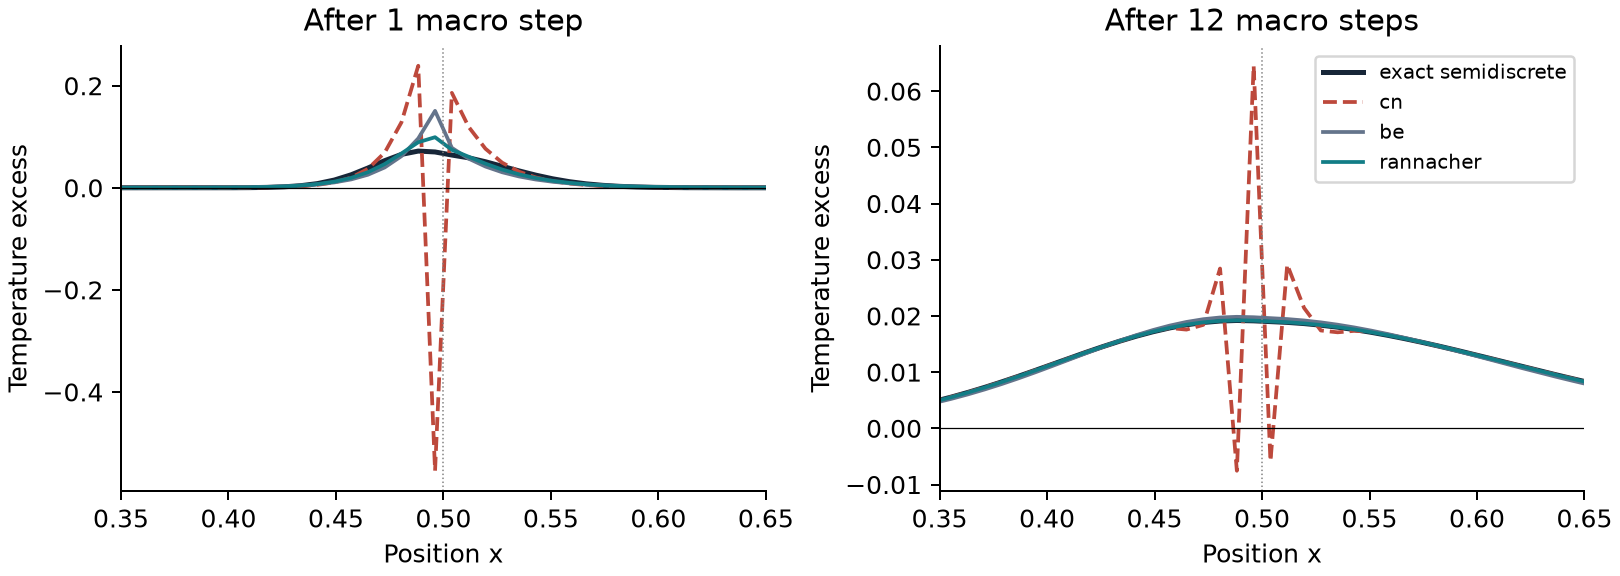
\includegraphics[width=\linewidth]{../examples/results/pulse.png}
\caption{Original pulse experiment. The reference solves the same discrete
ODE exactly in time, up to eigensolver roundoff. The dotted line marks the
material interface. Axes show a neighbourhood of the pulse.}
\label{fig:pulse}
\end{figure}
\begin{table}[ht]
\centering\small
\begin{tabular}{lrrr}\toprule
Method & First minimum & $E^1/E^0$ & Final time error\\\midrule
\PulseRows
\bottomrule\end{tabular}
\caption{Mass-weighted RMS error at $t=12\Delta t$ against the discrete
reference. Every table value is generated from recorded JSON outputs.}
\label{tab:pulse}
\end{table}
CN is energy stable but retains alternating short-scale modes
(Fig.~\ref{fig:pulse}). Startup reduces the final error by a factor of
$\Reduction$ relative to CN at this step size. The nonnegative minimum for
startup is an observation for these data, not a general theorem.

\newpage
\section{Verification and separation of errors}
The reference diagonalizes $S=M^{-1/2}KM^{-1/2}=Q\Lambda Q^T$ and computes
\begin{equation}\label{eq:exact}
 \boldsymbol T_h(t)=M^{-1/2}Qe^{-t\Lambda}Q^TM^{1/2}\boldsymbol T_0.
\end{equation}
Small negative eigenvalues caused by roundoff are clipped to zero. This
reference requires $O(N^2)$ eigenvector storage and is used for verification,
not as a large-scale solver. On a separate five-cell nonuniform heterogeneous
mesh, its maximum discrepancy from a dense matrix exponential is
$\ExpmError$. Tests also compare individual steps with dense linear solves
and the two-cell exchange mode with its closed-form amplification.

The reported norm is
$\|e\|_M=(\sum_i M_i e_i^2/\sum_i M_i)^{1/2}$.
Time error compares the numerical integrator to Eq.~\eqref{eq:exact} on the
fixed pulse mesh at $t=0.02$, using 20, 40, 80, 160 and 320 intervals.
The last refinement pair gives orders $\CNOrder$ (CN), $\BEOrder$ (BE)
and $\RanOrder$ (startup). Coarse CN errors are not in the asymptotic regime;
the full curves must be considered rather than a single fitted slope.

\begin{figure}[ht]
\centering
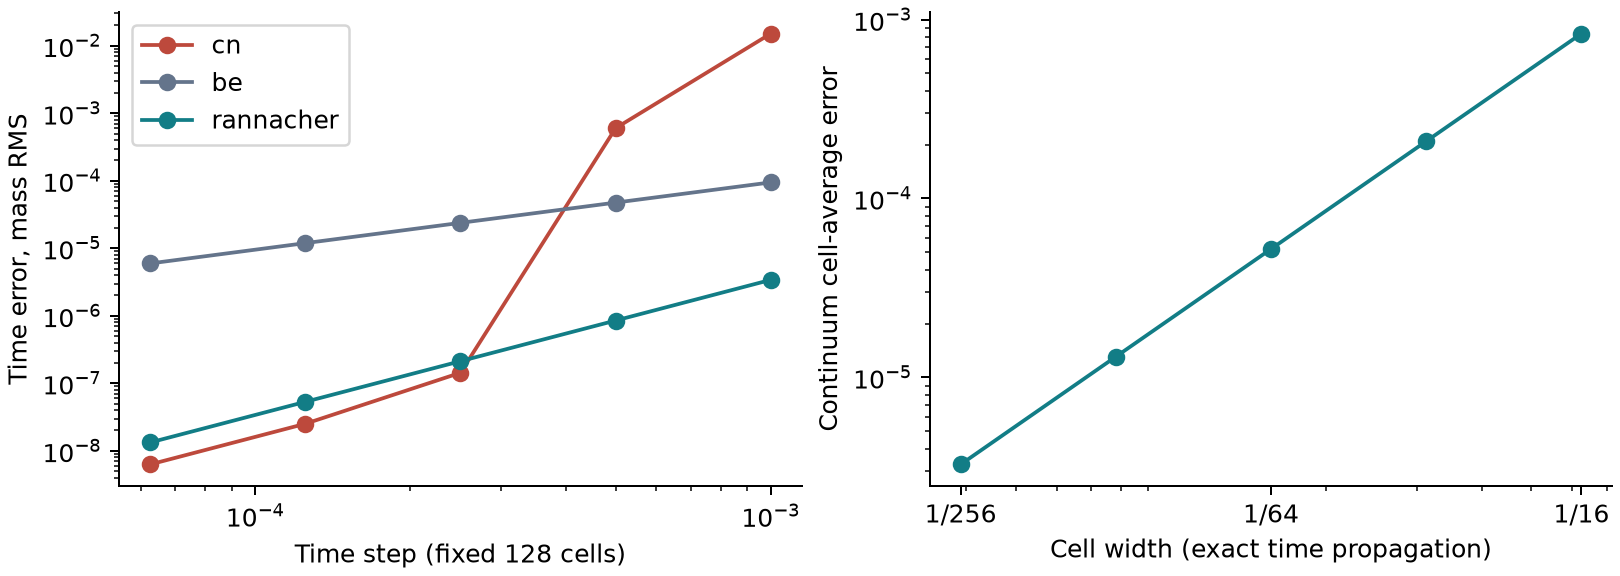
\includegraphics[width=\linewidth]{../examples/results/convergence.png}
\caption{Left: time error at fixed spatial discretization for the heterogeneous
pulse. Right: continuum cell-average error for a separate homogeneous cosine
experiment with exact discrete time propagation. These are different errors.}
\label{fig:convergence}
\end{figure}

To isolate space error, take homogeneous $k=c=1$ and the smooth solution
$T(x,t)=2+e^{-\pi^2t}\cos(\pi x)$. Initialize exact cell averages
$T_i(0)=2+\operatorname{sinc}(h/2)\cos(\pi x_i)$, where
$\operatorname{sinc}(s)=\sin(\pi s)/(\pi s)$, and compare Eq.~\eqref{eq:exact}
at $t=0.1$ with analytical cell averages. No time-stepping error is present.

\begin{table}[ht]
\centering\small
\begin{tabular}{rrr}\toprule
Cells & Cell-average space error & Order\\\midrule
\SpaceRows
\bottomrule\end{tabular}
\caption{Spatial refinement on the smooth homogeneous problem. Orders are
$\log_2(e_h/e_{h/2})$. The norm measures cell averages, not a reconstructed field.}
\end{table}

\newpage
\section{Discussion, reproducibility and limitations}
All three methods preserve heat within a maximum relative drift of
$\MaxDrift$ in the pulse experiment. Their quadratic energy decreases at
every recorded interval, but CN violates the lower temperature bound
(Fig.~\ref{fig:diagnostics}). Conservation and dissipation are therefore
necessary diagnostics that do not replace a componentwise bounds check.

\begin{figure}[ht]
\centering
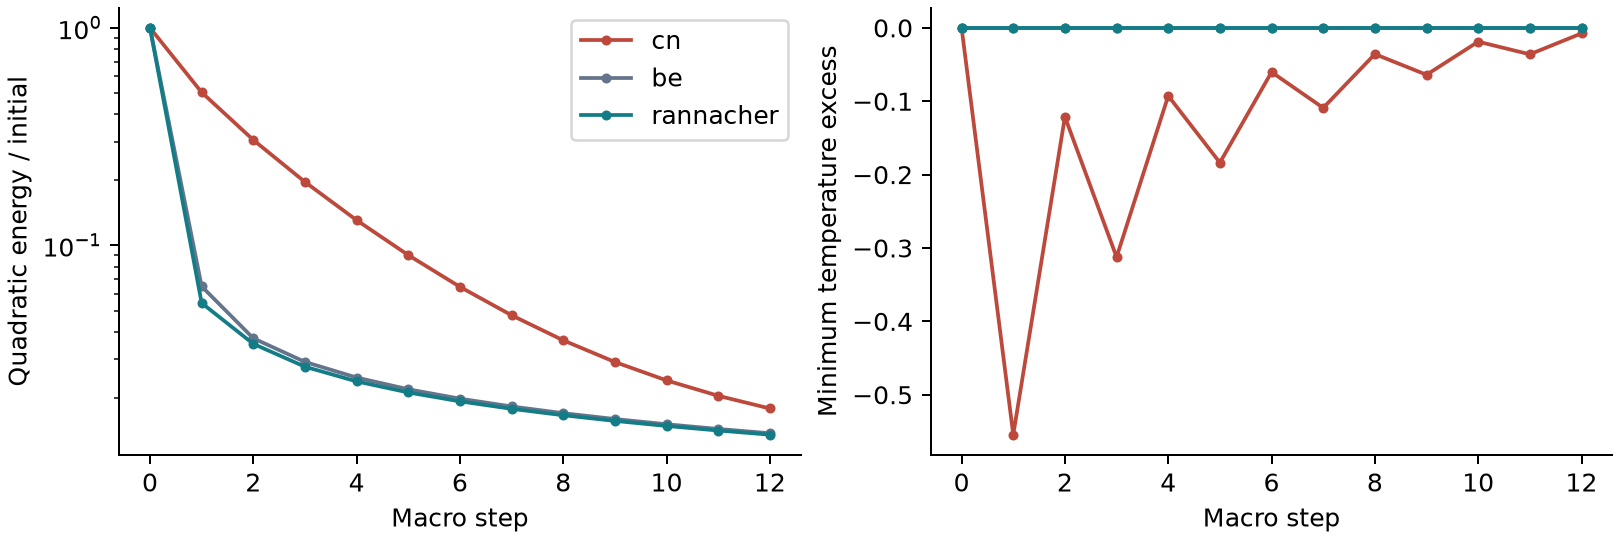
\includegraphics[width=.94\linewidth]{../examples/results/diagnostics.png}
\caption{Conservation of heat is checked separately in the data. Here all
three energy curves decrease, while only undamped CN produces a negative
temperature excess in the recorded pulse trajectory.}
\label{fig:diagnostics}
\end{figure}

For this discretization, $M+\theta\Delta tK$ has a nonnegative inverse.
A sufficient nonnegative-update condition is
$\Delta t\leq\min_i M_i/[(1-\theta)K_{ii}]$ for $\theta<1$.
BE has no such step restriction, and CN has the sufficient bound
$2\min_i(M_i/K_{ii})$. Exceeding this bound loses a guarantee but does not
prove every initial condition will undershoot. Similarly, a finite startup
attenuates stiff modes but cannot certify every subsequent CN step.

CN becomes more accurate than startup on the finest tested time grids;
startup is not a universal accuracy improvement. The smooth space experiment
verifies only the homogeneous cell-average problem, not interface accuracy,
arbitrary nonuniform meshes or physical experiments. Radiation, latent heat,
convection and temperature-dependent properties are omitted.

The CLI \texttt{heatstart -{}-output examples/results} reproduces complete CSV
histories, JSON metrics and figures. Scripts check all recorded values,
generate manuscript tables from JSON, compile LaTeX and enforce the page
cap. Hashes bind inputs to the PDF; every rendered page is visually inspected.

\section{Conclusion}
The heterogeneous pulse demonstrates that CN energy decay can coexist with
unphysical undershoot. Four BE half-steps reduce coarse-step time error while
retaining second-order convergence. Separate references distinguish discrete
verification from continuum error; physical validity remains untested.

\begin{thebibliography}{9}\small
\bibitem{rannacher} R. Rannacher. Finite element solution of diffusion problems
with irregular data. \emph{Numerische Mathematik} 43, 309--327, 1984.
\href{https://eudml.org/doc/132904}{Public bibliographic record}.
\bibitem{langtangen} H. P. Langtangen. \emph{Finite difference methods for
diffusion processes}. INF5620, 2014.
\href{https://hplgit.github.io/INF5620/doc/pub/H14/diffu/html/._main_diffu001.html}{Author's public notes}.
\end{thebibliography}
\end{document}
